\subsubsection{Advanced thread scheduling}

The \emph{main goal} of this section is to show how a CUDA kernel uses hardware execution resources: thread block allocation to execution resources, execution resource capacity constraints, and zero-overhead thread scheduling.

\highspace
In general, \textbf{CUDA thread blocks execute independently and can run in any order}. The hardware is \textbf{free to assign blocks to any processor at any time}. This flexibility allows the GPU to optimize resource utilization and balance the load. A kernel (the function that runs on the GPU) scales to any number of parallel processors. This means that the same code can run efficiently on GPUs with different numbers of cores.

\highspace
\begin{wrapfigure}{r}{0.35\textwidth}
    \centering
    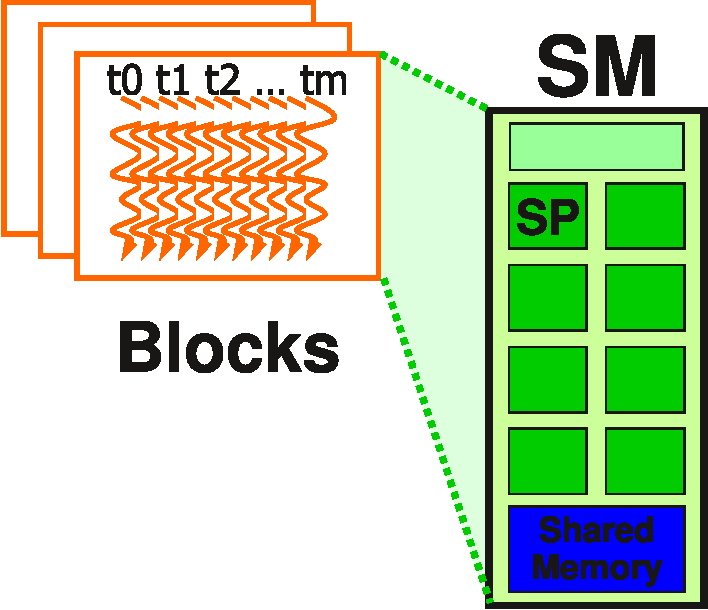
\includegraphics[width=0.34\textwidth]{img/executing-thread-blocks-1.pdf}
\end{wrapfigure}
Thread blocks are the basic unit of work in CUDA and are assigned to SMs in block granularity (as we saw in Chapter \ref{subsubsection: Running a CUDA program on a GPU}). This means that a \textbf{thread block cannot be split across multiple SMs, but is executed entirely within a single SM}. Each SM has a \emph{limit} on the number of threads and thread blocks it can support simultaneously. For example, the \textbf{Volta SM can handle up to 2048 threads}. The number of blocks an SM can hold depends on the number of threads per block:
\begin{itemize}
    \item If a block has 256 threads, up to 8 blocks can fit ($256 \times 8 = 2048$ threads).
    \item If a block has 512 threads, only 4 blocks can fit ($512 \times 4 = 2048$ threads).
\end{itemize}
The \textbf{SM manages the indexes of the threads and blocks assigned to it}, enabling scheduling and execution.

\highspace
\begin{flushleft}
    \textcolor{Green3}{\faIcon{bookmark} \textbf{Von Neumann model with SIMD units}}
\end{flushleft}\index{Von Neumann model with SIMD units}
The \textbf{Von Neumann Model} consists of a Control Unit, ALU (Arithmetic Logic Unit), Registers, Memory, and I/O components that work in a sequential manner. However, when we \textbf{integrate SIMD} (Single Instruction, Multiple Data) units into the model, we add the \textbf{ability to process multiple data items simultaneously using a single instruction}.

\highspace
As we have explained in the section \ref{subsubsection: Single Instruction, Multiple Data (SIMD) processor} page \pageref{subsubsection: Single Instruction, Multiple Data (SIMD) processor}, SIMD allows the same operation to be performed on multiple pieces of data in parallel. This means a Control Unit (CU) sends the same instruction to multiple ALUs, each working on different data at the same time.

\newpage

\begin{flushleft}
    \textcolor{Green3}{\faIcon{bookmark} \textbf{Von Neumann model with SIMD units in GPUs}}
\end{flushleft}
The \textbf{architecture uses SIMD units to execute multiple threads in parallel}, making GPUs highly efficient at tasks involving large data sets, such as image processing, matrix multiplication, and other data-parallel computations.

\highspace
In \textbf{CUDA}, \textbf{warps} (groups of 32 threads) are \textbf{executed in a SIMD fashion}. \textbf{All threads in a warp perform the same operation, but on different pieces of data}. This is critical for speeding up computations that need to process large amounts of data in parallel. SIMD capabilities allow GPUs to efficiently handle large numbers of parallel tasks, making them far more powerful than traditional CPUs for certain workloads, such as graphics rendering and scientific computing.

\begin{figure}[!htp]
    \centering
    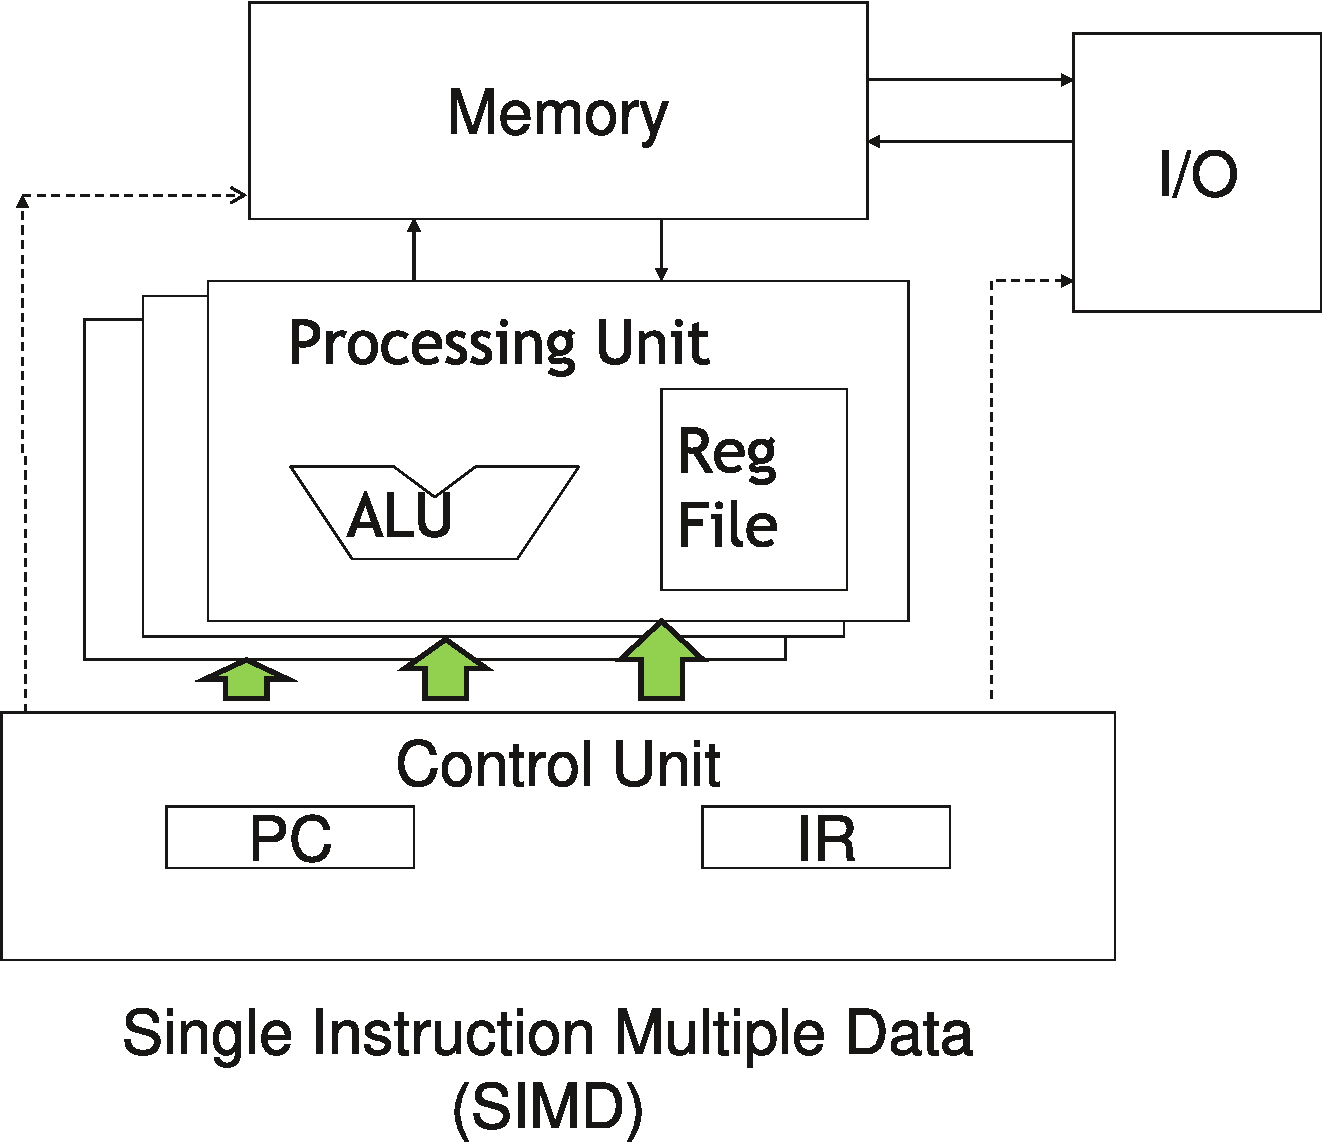
\includegraphics[width=.6\textwidth]{img/von-neumann-model-with-simd-1.pdf}
    \caption{Von Neumann model with SIMD units.}
\end{figure}